% This is samplepaper.tex, a sample chapter demonstrating the
% LLNCS macro package for Springer Computer Science proceedings;
% Version 2.21 of 2022/01/12
%
\documentclass[runningheads]{llncs}
%
\usepackage[T1]{fontenc}
% T1 fonts will be used to generate the final print and online PDFs,
% so please use T1 fonts in your manuscript whenever possible.
% Other font encondings may result in incorrect characters.
%
\usepackage{graphicx}
\graphicspath{ {./images/} }
% Used for displaying a sample figure. If possible, figure files should
% be included in EPS format.
%
% If you use the hyperref package, please uncomment the following two lines
% to display URLs in blue roman font according to Springer's eBook style:
%\usepackage{color}
%\renewcommand\UrlFont{\color{blue}\rmfamily}
%\urlstyle{rm}
%
\usepackage{float}

\begin{document}
%
\title{Artificial Storytellers: Evaluating LLMs as Game Masters in Role-Playing Games }
%
\titlerunning{Evaluating LLMs as Game Masters}
% If the paper title is too long for the running head, you can set
% an abbreviated paper title here
%
\author{
Bartłomiej Gawryszuk \and
Kacper Pytkiewicz \and
Szymon Jędrzejczak \and
Hubert Łoziński \and
Michał Palski \and
Kamil Pojedynek \and
Jakub Watała \and
Jakub Kartkowski
}
%
\authorrunning{B. Gawryszuk et al.}
% First names are abbreviated in the running head.
% If there are more than two authors, 'et al.' is used.
%
\institute{Scientific club TK Games, Wrocław University of Science and Technology 
\email{pwrtkgames@gmail.com}\\
}
%
\maketitle              % typeset the header of the contribution
%
\begin{abstract}
Large Language Models (LLMs) have demonstrated remarkable versatility across numerous domains, with their applications in games and entertainment being actively explored by researchers and game developers. This paper evaluates the performance of LLM agents in assuming the role of Game Master (GM) for tabletop role-playing games (TTRPGs). We evaluated DeepSeek V3 across two custom-designed RPG systems: a Narrative System focused on storytelling and a Tactical Combat System with complex rules and statistics. Performance was assessed across six criteria, which measure narrative coherence, memory, adherence to rule sets, misuse resistance, creativity, and entertainment value. A case study was also performed on participants with varied experience in role-playing games. Our findings indicate that LLMs show promising potential as alternatives to human GMs, with particular strengths in narrative-driven gameplay scenarios, though they still face challenges with maintaining complex rule systems and tactical gameplay. This research contributes to the ongoing exploration of AI applications in gaming and interactive storytelling, highlighting both the capabilities and current limitations of LLMs in creating and leading immersive role-playing experiences.

\keywords{LLM  \and Role-playing games \and Artificial Intelligence in games.}
\end{abstract}
%
%
%
\section{Introduction}
A role-playing game (RPG) is a type of game in which players assume the role of a fictional character and experience the imagined stories involving such characters. Most such games involve a designated player, traditionally called the Game Master (GM) or the Dungeon Master (DM), who acts upon the actions of other players. Due to their versatility, LLMs have been found applicable in emulating the RPG experience in computer form. However, the challenges stem from the fact that the GM must creatively account for player agency.
This paper examines the results of our study concerned with using LLM-powered agents to run a text-based role-playing game, where such agents fill the role of a GM. In the study, data on player satisfaction with the experience and agent consistency with designer-given guidelines was collected and evaluated. 


\section{Related work}
There has been much research into the usage of large language models (LLMs) in tabletop role-playing games (TTRPGs) in the role of dungeon master (DM) or game master (GM), with the goal of testing the capabilities of artificial intelligence (AI) tools in this field. These studies were mainly focused on verifying whether LLMs can correctly and faithfully act as a DM/GM, which involves maintaining narrative coherence, immersing players into the story, being able to adapt to the players’ decisions, etc. A study by Pavlos Sakellaridis found that fine-tuning ChatGPT with the Critical Role Dungeons and Dragons Dataset \cite{ref_5} resulted in an increase in response quality and overall capabilities \cite{ref_2}. Similar improvements were found in a 2022 study by Callison-Burch et al. involving training Google’s LaMDA model on games played by human players and DMs from the D\&D Beyond forum \cite{ref_3}. Some other approaches which yielded better results in this area were splitting an LLM’s responsibilities onto multiple AI agents in addition to fine-tuning, as shown in a 2025 study by Jørgensen et al. \cite{ref_4}. Generally, in contrast to an experienced human DM, LLMs were found to have difficulties with communicating essential information, presenting sufficient danger and challenges to the players \cite{ref_2}. In his research, Tuul Triyason points out that even though the narrative generated by AI was coherent, it was lacking in depth and immersive qualities \cite{ref_1}. The limitations stemming from the fact that LLMs offer a purely text-based form of interaction prevented players from becoming fully immersed in the fictional worlds of TTRPGs. Players highlighted the importance of factors such as tone of voice and facial expressions in real-life TTRPG sessions, which LLMs are currently not able to replicate \cite{ref_1}. Overall, it was found that at the time of publication of the aforementioned articles, AI was not considered ready to fully replace human DMs/GMs, but could offer help for novice DMs/GMs \cite{ref_1,ref_2,ref_3,ref_4}.

\section{Proposed methodology}
In this section, we provide an overview of the methodology we used to evaluate the performance of Large Language Models (LLMs) in the role of Dungeon Master for tabletop Role-Playing Games (RPGs). We will outline the selection of LLMs used for our experiment, the methodology used during the experiment, and the system we developed to objectively evaluate the performance of the selected LLMs.
\subsection{LLM selection}
After careful testing and consideration of many different LLMs, we decided to use DeepSeek V3 \cite{ref_6}, which is a popular state-of-the-art LLM with 671 billion parameters. We have also evaluated many smaller models from the Llama family, as well as Gemma 3, Mistral, and DeepSeek-R1 distillations. However, we found that their performance was not satisfactory due to failures in producing coherent narratives and instruction following.
\subsection{Experiment setup}
Our experiment was split into 2 phases. During the first phase, the setup was evaluated by three players from the research team who already had experience with traditional role-playing games. We polished the instructions and our scenario with feedback from the tests. The second phase involved performing an experiment on various volunteers during Wroclaw University of Science and Technology's Open Day. The participants were mostly high school students.

\subsubsection{Experiment on research team}
The first experiment was carried out with our research team as players. In order to have full control over the course of the experiment, we prepared a custom campaign, which contains a very simplified iteration of a D\&D style combat system and character creation. The results of certain actions are determined by dice rolls. For this experiment, the player is meant to roll the dice and tell the DM the result. The campaign was designed to support 30-minute sessions---however, this duration may vary greatly depending on the players' choices and their rolls' outcomes. We decided to prepare two different RPG systems to compare how LLMs deal with different aspects of the role-playing game. The first system, the \textbf{Narrative System}, is designed to focus on telling a story, without complex rules. The other system is called the \textbf{Tactical Combat System}---it offers more attributes, skills, statistics, tracking of items, status effects, etc. It also specifies rules for combat with mechanics of turns, actions per turn, and many special moves. A script containing an outline of the story and the rules of the system is used as the first prompt for the LLM at the beginning of the session. Each person taking part in this experiment played multiple sessions in both systems. Afterwards, the players would fill an advanced questionnaire which aimed to gather comprehensive feedback from the players. 

\subsubsection{Experiment on participants}
The second experiment was carried out by the research team on volunteering participants. They were presented with a desktop application created by the research team members. Crucially, the application did not share system prompts and offered a more immersive experience with stylized visuals. It also was able to detect if a session had ended by finding an appropriate flag in the AI's response. To accommodate for this, a modification was made to the system instructions which detailed when and where to use this flag. In this experiment, we decided to use the Narrative System only, with the goal of lowering the knowledge and expertise requirements needed to play. Each participant was given about 30 minutes to play. After the end of each session, the role-playing transcript was saved for further analysis, and participants were redirected to a simplified questionnaire. 

\subsection{System for performance evaluation}
We devised two bespoke systems to evaluate the performance of the selected LLM during each session through questionnaires. A more advanced system was used for our research team because we spent much more time playing role-playing sessions with AI while volunteering participants played only one session. However, the experience of playing RPGs can't be accurately described only in numbers, so in both questionnaires we provided a space for participants to share their additional comments and errors or unexpected behavior encountered. This question was crucial for the evaluation process.

\subsubsection{Advanced Questionnaire}
The overall performance is assessed across six criteria that we consider important for an LLM DM, each of which shall be graded with a score from 1 to 10:

\begin{description}
    \item[Narrative Coherence]
    Measures the ability of an LLM to follow basic narrative structure, rules of causality, and keep characters coherent.
    \item[Memory]
    Measures the ability of an LLM to retain correct data such as character names or player statistics.
    \item[Adherence to the Rule Set]
    Measures the ability of an LLM to correctly follow the rules and script provided at the beginning of the session.
    \item[Misuse Resistance]
    Measures the ability of an LLM to resist misuse. We define \textit{misuse} in this context as a deliberate attempt by the player to force the LLM into failing one or more of the criteria listed.
    \item[Creativity]
    Measures the ability of an LLM to create unusual and amusing scenarios, as well as the ability to adapt to player actions.
    \item[Entertainment Value]
    Measures how much amusement the player got from the session. A key characteristic of a game is that it is fun, and games which do not provide enough entertainment value are not considered \textit{good} games. By extension, we shall consider a failure to provide enough entertainment for the player as a failure on the DM's part. 
\end{description}


\subsubsection{Simplified Questionnaire}
The questionnaire starts with questions about the participant's experience with role-playing games. The overall performance is assessed across three mandatory criteria and one optional criterion.

\begin{description}
    \item[Gameplay Satisfaction]
    Measures how much entertainment and amusement player felt after the session, on a scale from 1 to 5.
    \item[Model Creativity]
    Measures the ability of the LLM DM to create unusual and amusing scenarios, as well as the ability to adapt to player actions, on a scale from 1 to 5.
    \item[Story Adherence]
    Measures how much of the story was logical and whether it didn't contradict itself, on a scale from 1 to 4.
    \item[Comparison with Human Game Master]
    Measures to what extent the LLM DM can provide a similar experience, on a scale from 1 to 5, where a rating of 1 meant much worse, a rating of 3 meant the same and a rating of 5 meant much better. This question was optional and asked only if the participant had experience with role-playing games beforehand.
\end{description}

\section{Evaluation}
\subsection{Researchers as players}
We evaluated DeepSeek V3's performance during multiple sessions using the two systems we devised, and assessed its capabilities as a competent DM in accordance with the criteria defined. Our experiments yielded the following results:


\begin{enumerate}
\item The Narrative System yielded better results in the \textit{Narrative Coherence} criterion than the Tactical Combat System, because the DM has less things to take into account when creating story.
\item The Narrative System yielded better results in the \textit{Memory} criterion than the Tactical Combat System, because there was less crucial information to remember by the DM, therefore there were less opportunities to make a mistake. 
\item The Narrative System yielded slightly better results in the \textit{Adherence to the Rule Set} criterion than the Tactical Combat System, because DM had trouble implementing numerous rules at the same time. 
\item The Tactical Combat system yielded better results in the \textit{Misuse Resistance} criterion than the Narrative System, because less regulations in the Narrative System resulted in more opportunities for the player to confuse the DM.
\item The Narrative System yielded drastically better results in the \textit{Creativity} criterion than the Tactical Combat System. The responses were much longer, were written vividly and were much more interesting. 
\item The Narrative System yielded better results in the \textit{Entertainment Value} criterion than the Tactical Combat system due to the absence of frustrating mistakes and the DM not remembering basic facts and the overall narrative.
\end{enumerate}
Using the Narrative System allows the DM to come up with a passable story. We also observed that with this system, the DM was able to adapt to the player's actions in a meaningful way. However, it fell short in the aspect of mechanical depth.
The Tactical Combat System allows the DM to present advanced tactical scenarios to the player. Unfortunately, the DM made a significant number of mistakes during gameplay and failed to provide an engaging story.

\begin{table}
    \centering
    \caption{Average scores from researchers}
    \label{tab:research-team-scored}
    \begin{tabular}{|c|c|c|}
        \hline
        Category & Tactical Combat System & Narrative System \\
        \hline
        Narrative Coherence & 6.33 & 6.67 \\
        \hline
        Memory & 5.33 & 6.67 \\
        \hline
        Adherence to Rule Set & 4.67 & 5.33 \\
        \hline
        Misuse Resistance & 5.00 & 4.33\\
        \hline
        Creativity & 5.33 & 6.67 \\
        \hline
        Entertainment Value & 7.00 & 8.33 \\
        \hline
    \end{tabular}
\end{table}

\subsection{Volunteers as players}
We evaluated DeepSeek V3's performance as an LLM DM on a group of volunteers. We received 27 chat logs and 25 filled-in questionnaires. This experiment yielded the following results, showcased in Figures \ref{fig:volunteer-gameplay}, \ref{fig:volunteer-creativity} and \ref{fig:volunteer-human}:
\begin{figure}[H]
    \centering
    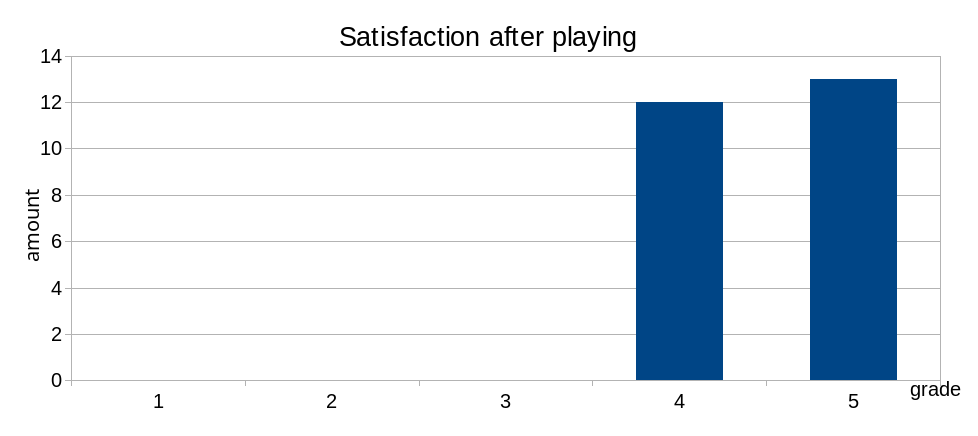
\includegraphics[width=.85\textwidth]{images/satisfaction.png}
    \caption{Volunteer ratings of their gameplay satisfaction.}
    \label{fig:volunteer-gameplay}
    
    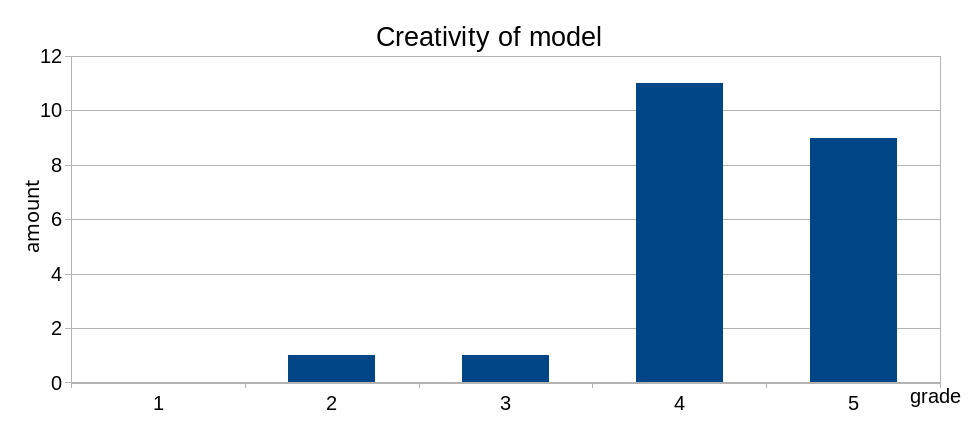
\includegraphics[width=.85\textwidth]{images/creativity.png}
    \caption{Volunteer ratings of the LLM's creativity.}
    \label{fig:volunteer-creativity}

    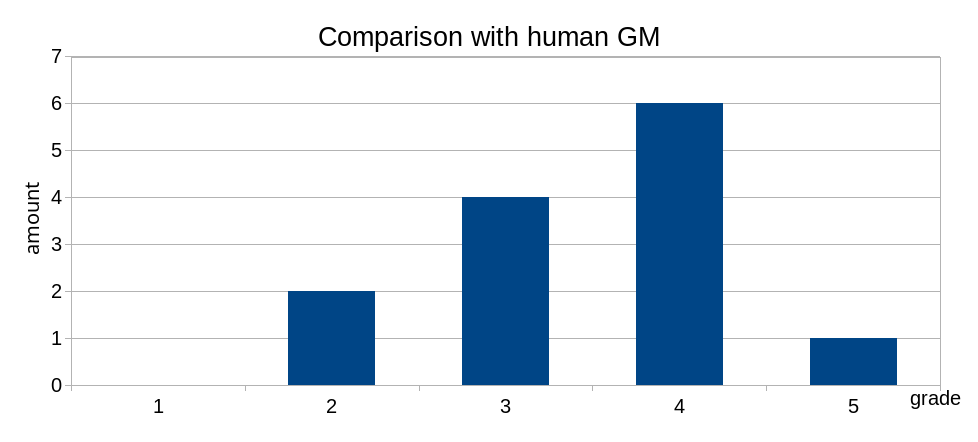
\includegraphics[width=.85\textwidth]{images/comparision with human.png}
    \caption{Volunteer comparison with a human GM.}
    \label{fig:volunteer-human}
\end{figure}

\noindent
From the data we gathered, we drew the following conclusions:
\begin{description}
    \item[Positive general impressions] The general impression of the participants was positive. It mirrors our initial impression during the start of the research. Because participants had the opportunity to play only one session, we suspect that the general positivity towards the DeepSeek performance stems from the "novelty effect". The fact that an LLM is capable of carrying an RPG session was impressive enough for them. However, they did not have the opportunity to play more sessions to form a more nuanced opinion. 
    \item[Weak adherence to the scenario] Participants were often able to go off-script, regardless if they did it intentionally or not. The DM made no attempts to prevent these occurrences from happening. It happened much more often than during our first experiment---we suspect that this was because we knew the script well and therefore subconsciously followed it.
    \item[Reliability issues] DeepSeek proved to be too unreliable to be integrated into a more sophisticated RPG game system. Our setup exhibited considerable amounts of latency in the DeepSeek API calls, which disrupted the gameplay experience. Moreover, the mechanism for ending the session was unpredictable and often led to situations where sessions ended abruptly in places it shouldn't have. It was such a disruptive issue that we had to remove it from the desktop application during the experiment. A solution to this problem would to be use proper tool-calling with a model that supports it. Unfortunately DeepSeek V3 has no tool-calling support.
\end{description}

\subsection{Arithmetic and data insertion errors}
During gameplay, the LLM sometimes made significant arithmetic and logical mistakes. Below are a few excerpts from sessions conducted during our experiments that showcase these issues.

\subsubsection{Difficulty with adding and subtracting numbers}
The model sometimes made arithmetic errors in areas involving damage calculation. The following excerpt showcases this:
\begin{quote}
    \textbf{Player}: I roll 15.\\
    \textbf{DM}: Kris rolls a d20 and adds their Strength (+3).\\
    They need to beat the Marauder Leader’s Dodge of 11.\\
    Kris rolls a 15 + 3 = 18. That’s a hit!\\
    Damage Roll: Kris’s longsword deals d8 damage. They roll a 6. \\
    The Marauder Leader has 2 Armor, so he takes 4 damage.\\
    The Marauder Leader’s HP drops from 12 to 4.
\end{quote}
\noindent
During the damage calculation, the model subtracts 4 from 12 and it erroneously sets the Marauder Leader's health points to 4. The correct number should be 8.

\subsubsection{Difficulty with comparing numbers}
Sometimes the model would make comparison errors between two numbers, for example during dice roll evaluation.
\begin{quote}
    \textbf{DM}: Bandit Swordsman’s Turn\\
    The Bandit Swordsman takes advantage of your failed disarm 
    attempt and swings his sword at you.\\
    Attack Roll: The swordsman rolls a d20 and adds his Strength (+3). 
    He needs to beat your Dodge of 14.\\
    He rolls a 10 + 3 = 13. That’s a hit! 
\end{quote}
\noindent
In this excerpt, the attack roll would only succeed if at least 14 was rolled. However, when comparing dice rolls, the model erroneously decides 13 is greater than 14, and the roll wrongly succeeds. 

\subsubsection{Accepting and justifying incorrect input data}
We also observed that the model wouldn't correct the player if they entered malformed input data. In this example, the player was asked to roll two dice, but they only entered the value of one roll:
\begin{quote}
    \textbf{DM}: Kris is attempting to lull the creatures to sleep. \\
    This is a Very Hard (15) Charisma check. Since        
    Kris has the Performance talent, they roll with advantage 
    (roll twice and take the higher result).\\
    Let me know Kris’s Performance check and Susie’s action, and 
    we’ll continue the fight!\\
    \textbf{Player}: I rolled 4.\\
    \textbf{DM}: Roll 1: 4 + Charisma (+2) = 6\\
    Roll 2: (Not needed, since the first roll fails). 
\end{quote}
\noindent
When given one input, the model didn't ask for the remaining one, even if it could have altered the game in favor of the player.

\subsection{Randomness of rolls}
During testing, we observed a lack of variety in roll values generated by the LLM. Also, the values never reached the minimum value of 1 or the maximum value of 20, which made critical failure or critical success impossible. In a real-life RPG session, it is crucial for rolls to be truly random to not give anyone an advantage.

After counting individual rolls, our suspicions were proved true; values showed a non-uniform distribution and were oscillating near 12. We compared DeepSeek's rolls with the roll value distribution of a 20-sided die, which ideally should be uniform. We found that DeepSeek's roll distribution was vastly different, as shown in Figure \ref{fig:d20-roll-values} -- its rolls were not distributed uniformly and showed bias towards higher roll values.

\begin{figure}
    \centering
    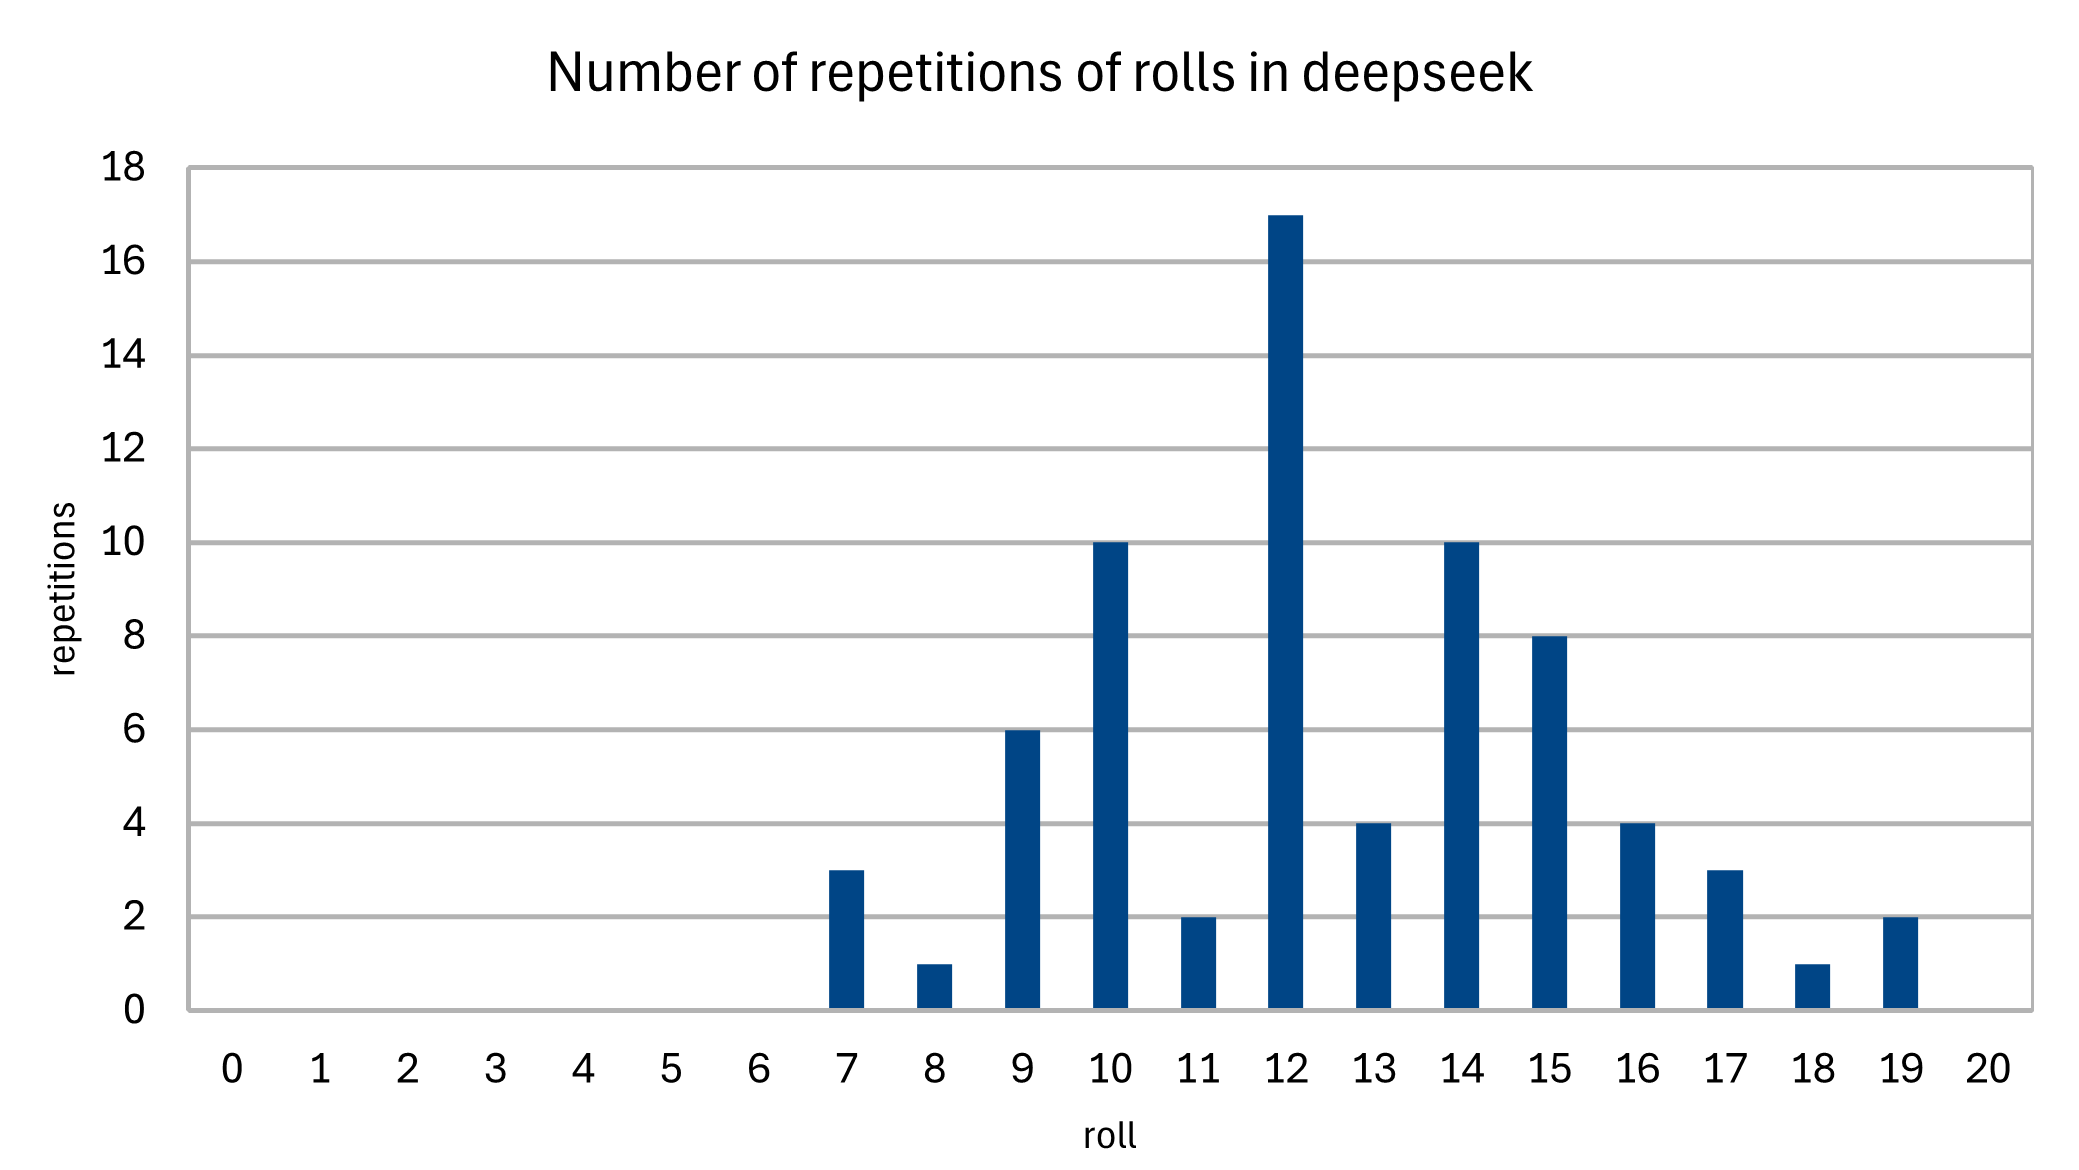
\includegraphics[width=\textwidth]{images/repetitions_final.png}
    \caption{Histogram of random 20-sided die roll values made by DeepSeek.}
    \label{fig:d20-roll-values}
\end{figure}


\subsection{Other issues}
The other issues we encountered during the evaluation process were:
\begin{description}
    \item[Not following prepared scenario] The LLM DM tended to forget about certain events and made up new ones.
    \item[Bloat] The LLM tended to generate long paragraphs that contained very little relevant information and were mostly padding. It was difficult to understand what the DM wanted the player to do. Occasionally, it wanted the player to do multiple actions simultaneously. Reading through these responses could be tedious.
    \item[Repetitive style] After having played multiple sessions, it became clear that the descriptions generated by the LLM were very repetitive, making them progressively less interesting and novel.
\end{description}

\section{Conclusions}
Our research indicates that despite promising first impressions, upon further inspection, LLMs fulfilling the role of Game Masters display a lot of issues. Many of them can be resolved to some extent by applying better prompting techniques and incorporating them as part of a bigger application. However, the latter proved to be difficult and unreliable, limiting the potential of this technology. Other important issues, such as the lack of creativity and general predictability, as well as the tendency to ignore set rules and scenarios and vulnerability to misuse cannot be solved, as they are inherent flaws of LLM technology. Humans are not prone to these issues, making them superior to LLMs in terms of Game Master capabilities, and therefore it is not yet recommended to fully rely on Large Language Models as of the time of publication of this article.

\begin{credits}
\subsubsection{\ackname} We are deeply grateful to M.Eng. Weronika Węgier and M.Eng. Szymon Wojciechowski for all the guidance, support, and expertise provided to the team. Without their help, not only on this particular project but throughout the term of their supervision, this would simply not be possible.

\subsubsection{\discintname}
The authors have no competing interests to declare that are
relevant to the content of this article.
\end{credits}
%
% ---- Bibliography ----
%
% BibTeX users should specify bibliography style 'splncs04'.
% References will then be sorted and formatted in the correct style.
%
% \bibliographystyle{splncs04}
% \bibliography{mybibliography}
%
\begin{thebibliography}{8}
\bibitem{ref_1}
Tuul Triyason. 2023. Exploring the Potential of ChatGPT as a Dungeon Master in Dungeons \& Dragons tabletop game. Published on ACM Digital Library.

\bibitem{ref_2}
Pavlos Sakellaridis. 2024. Exploring the Potential of LLM-based Agents as Dungeon Masters in Tabletop Role-playing Games. Published in the Utrecht University Student Theses Repository.

\bibitem{ref_3}
Chris Callison-Burch, Gaurav Singh Tomar, Lara J. Martin, Daphne Ippolito, Suma Bailis and David Reitter. 2022. Dungeons and Dragons as a Dialog Challenge for Artificial Intelligence. Published on ACL Anthology.

\bibitem{ref_4}
Nicolai H. Jørgensen, Sarmilan Tharmabalan, Ilhan Aslan, Nicolai Brodersen, Hansen and Timothy Merritt. 2025. Static Vs. Agentic Game Master AI for Facilitating Solo Role-Playing Experiences. Published on arXiv.

\bibitem{ref_5}
Revanth Rameshkumar, Peter Bailey. 2020. Storytelling with dialogue: A Critical Role Dungeons and Dragons Dataset. Published on ACL Anthology.

\bibitem{ref_6}
Aixin Liu et al. 2024. DeepSeek-V3 Technical Report. Published on arXiv.

\end{thebibliography}
\end{document}
